\section{Trattazione metodologica}

\subsection{Ambiente di sviluppo}

\subsubsection{Hardware e software richiesti}
Come anticipato,i software Isaac Sim e Isaac Lab sono richiesti per lo scopo del progetto, oltre a Visual Studio Code per la stesura del codice Python, la redazione di file YAML, XML e vari altri. I requisiti più stringenti sono quelli richiesti da Isaac Sim e Isaac Lab. Secondo la documentazione \cite{nvidiaIsaacSim2025}, le specifiche minime della postazione sono 32 GB\footnote{per l'uso avanzato se ne richiedono 64} di RAM, 4 core, 50 GB di memoria di archiviazione ed una scheda GeForce RTX 3070 con 8 GB di VRAM, le specifiche consigliate sono ben più alte. Per soddisfare questi requisiti si è scelto di svolgere il progetto su una macchina virtuale provvista di CPU a 16 core, GeoForce RTX 3090\footnote{dalle specifiche la scheda ha 24 GB di VRAM}, circa 350 GB di memoria di archiviazione e 24 GB di RAM. La scelta del sistema operativo è ricaduta su Ubuntu 22.04 per la  sua compatibilità sia con Isaac Sim che con ROS (illustrato di seguito). Isaac Sim e Isaac Lab appartengono alla suite Omniverse di Nvidia e richiedono diversi driver come CUDA per funzionare correttamente. Una volta installati, si è reso necessario un periodo di formazione sulla piattaforma Nvidia Learn per apprendere le basi di creazione degli scenari di simulazione, importazione degli asset\footnote{robot, sensori e scenari open source} e apprendimento di politiche di reinforcement learning. Il corso è disponibile online sulla piattaforma dedicata e si compone delle seguenti lezioni:
\begin{itemize}
    \item Getting Started: Simulating Your First Robot in Isaac Sim
    \item Ingesting Robot Assets and Simulating Your Robot in Isaac Sim
    \item Synthetic Data Generation for Perception Model Training in Isaac Sim
    \item Developing Robots With Software-in-the-Loop (SIL) In Isaac Sim
    \item Leveraging ROS 2 and Hardware-in-the-Loop (HIL) in Isaac Sim
\end{itemize}
Secondo le nozioni offerte nel corso, l'addestramento robotico in Isaac Lab si articola, tipicamente, nelle tre fasi seguenti:
\begin{enumerate}
    \item Design: costruzione e modifica dell'ambiente e dei sistemi meccanici.
    \item Tune and train: simulazione dei sistemi fisici e della sensoristica virtuale. Replicator genera i dati sintetici coerenti con la simulazione, Omnigraph opera il tuning dei parametri fisici per rendere lo scenario realistico e Isaac Lab si occupa dell'addestramento dell'agente tramite reinforcement learning.
    \item Deploy: il sistema viene messo in opera attraverso delle API ROS.
\end{enumerate}

Sulla base dei passaggi appena descritti, la documentazione di Isaac Lab propone due flussi di lavoro. Il primo (vedi Figura \ref{fig:isaac_lab_dir_wf}) viene detto Direct Workflow e prevede, una volta definito l'ambiente, la composizione di uno script che caratterizza gli elementi del Markov Decision Process (stati, azioni e ricompense) e la logica implementativa rispetto all'agente e all'evoluzione dello scenario. Lo script unico impone una natura monolitica che semplifica l'architettura ma rende il codice più rigido e il debug più complesso. Questo approccio è particolarmente consigliato agli utenti che hanno familiarità con Isaac Gym, il framework per l'apprendimento in simulazione utilizzato prima dell'avvento di Isaac Lab.

\begin{figure}[h]
    \centering
    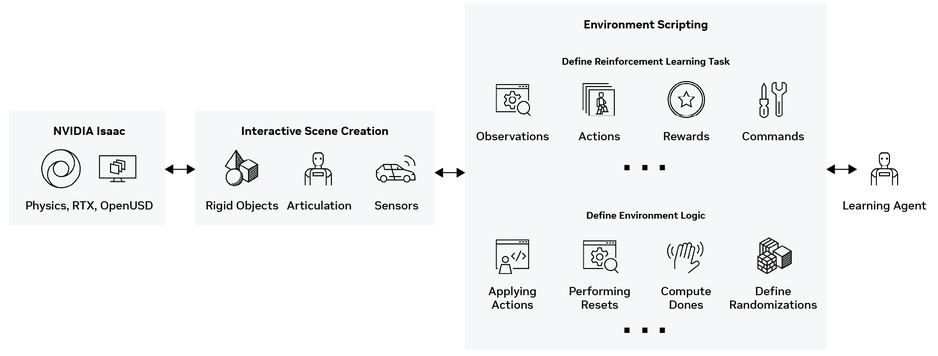
\includegraphics[width=0.95\linewidth]{immagini/isaac_lab_dir_workflow.png}
    \caption{Workflow diretto. Fonte: \cite{nvidiaIsaacLab2025}}
    \label{fig:isaac_lab_dir_wf}
\end{figure}

Il secondo approccio viene chiamato Manager-based Workflow e si basa sulla scomposizione dell'architettura in entità dette "manager" che gestiscono le varie responsabilità in maniera modulare: 

\begin{itemize}
    \item Event manager: si occupa della randomizzazione delle variabili dello scenario come le posizioni degli ostacoli, i materiali, l'illuminazione ed altri aspetti che servono a migliorare le capacità di generalizzazione del modello.
    \item Observation manager: gestisce le misurazioni propriocettive ed esterocettive raccolte dai sensori virtuali del robot.
    \item Action manager: racchiude una descrizione dettagliata dello spazio dei giunti utile a calcolare in tempo la cinematica del robot e rapportarla alle azioni che l'agente compie.
    \item Curriculum manager: permette di organizzare i compiti e gli ambienti in ordine crescente di difficoltà, rendendo l'addestramento degli agenti più efficiente e robusto.
    \item Command manager: è l'entità dedicata al calcolo della posa del robot e delle velocità dei giunti in riposta al controllo.
    \item Reward manager: si occupa di calcolare ed archiviare le ricompense raccolte.
    \item Termination manager: ha l'incarico di terminare gli episodi di simulazione quando necessario.
\end{itemize}
Questa scomposizione permette di omettere la definizione delle interazioni tra gli elementi nello scenario e concentrarsi solo sulla caratterizzazione dello spazio degli stati, di quello delle azioni e delle ricompense.

\begin{figure}[h]
    \centering
    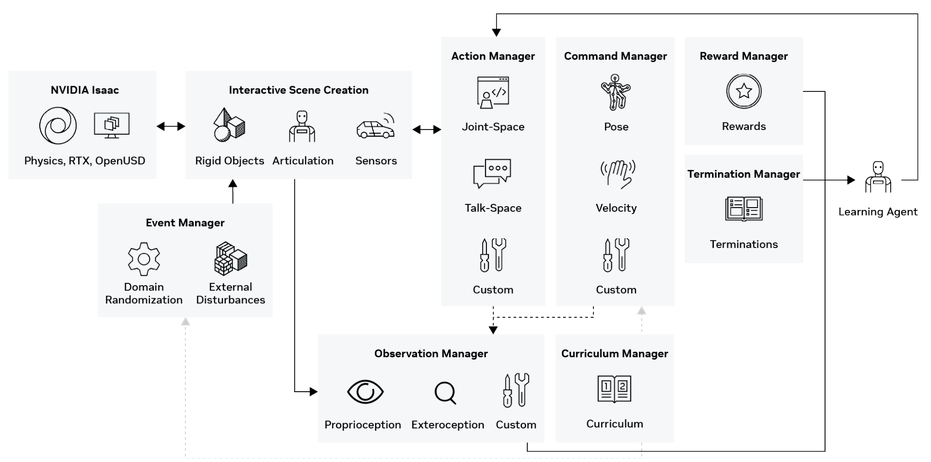
\includegraphics[width=0.95\linewidth]{immagini/isaac_lab_man_bas_workflow.png}
    \caption{Workflow manager-based. Fonte: \cite{nvidiaIsaacLab2025}}
    \label{fig:isaac_lab_man_bas_wf}
\end{figure}

Entrambi i workflow hanno una repository GitHub dedicata da cui è possibile ricavare esempi esplicativi delle varie componenti. L'approccio Manager-based può essere più complesso all'inizio dello sviluppo, ma è consigliato agli sviluppatori che si approcciano per la prima volta ad Isaac Lab.

Per trasporre le politiche elaborate durante le simulazioni nell'ambito reale ci si è avvalsi di ROS, il framework più usato per la scrittura di software robotico; si distingue per una struttura \textit{publish-subscribe} che modella l'interazione di sensori e attuatori con l'unità centrale di calcolo. In particolare si è scelta la versione ROS2 Humble per la compatibilità con gli strumenti utili allo scopo. ROS si è rivelato utile anche nelle prime fasi di allestimento dell'ambiente simulativo per interagire con il robot importato nello scenario Isaac Sim. Le specifiche hardware richieste sono trascurabili rispetto a quelle riportate in precedenza per i software Nvidia.

\subsubsection{Organizzazione del progetto e versionamento}

% struttura directories 
Il progetto è organizzato in diverse cartelle e sottocartelle per esigenze di modularità e ordine. Di seguito, si illustra la disposizione finale dell'ambiente:

\begin{itemize}
    \item \texttt{assets}: contiene le descrizioni USD delle varianti del G1.
    \item \texttt{checkpoints}: a sua volta racchiude \texttt{logs} e \texttt{model} in cui vengono salvate rispettivamente i log di simulazione e il modello finale derivante dall'addestramento.
    \item \texttt{configs}: racchiude i file di configurazione dell'agente, dell'ambiente e della politica, utilizzati per personalizzare l'addestramento.
    \item \texttt{managers}: raccoglie tutti i manager per la struttura ManagerBased (action, command, curriculum, event, observation, reward, termination). Al suo interno è stata creata una cartella per le funzioni MDP personalizzate.
    \item \texttt{models}: ospita modelli di computer vision utilizzati per contribuire alle osservazioni.
    \item \texttt{robot}: contiene i file di configurazione del robot e dei suoi attuatori.
    \item \texttt{scenes}: raccoglie le descrizioni degli scenari di simulazione.
    \item \texttt{scripts}: ci sono gli script di avvio per l'addestramento e per il test.
    \item \texttt{sensors}: ospita le descrizioni dei sensori montati sul robot.
    \item \texttt{task}: contiene la caratterizzazione del task specifico di evitamento ostacoli.
\end{itemize}

% versionamento GitHub


\subsection{Importazione del robot}

\subsubsection{Importazione URDF}
Come descritto in precedenza, Isaac Sim sfrutta il formato standardizzato di descrizione per le scene USD, ma la stragrande maggioranza degli asset robotici open source è nel formato URDF. Il software offre un convertitore tra i due formati che permette di importare nello spazio di lavoro molte delle risorse reperibili online. In prima istanza si è scelto di utilizzare la versione dell'umanoide G1 inclusa nelle librerie native di Isaac Sim, ma, già da un primo sguardo, è balzato all'occhio che il modello proposto avesse una sorta di "maschera" nella cavità inferiore della testa (visibile in Figura \ref{fig:confronto_g1}) che occludeva gran parte dello spazio di visione del LiDAR. Ritenendo questo impedimento non accettabile, si è preferito importare una versione diversa del robot trovata in una repository GitHub dedicata ai prodotti Unitree. 

\begin{figure}[h]
    \centering
    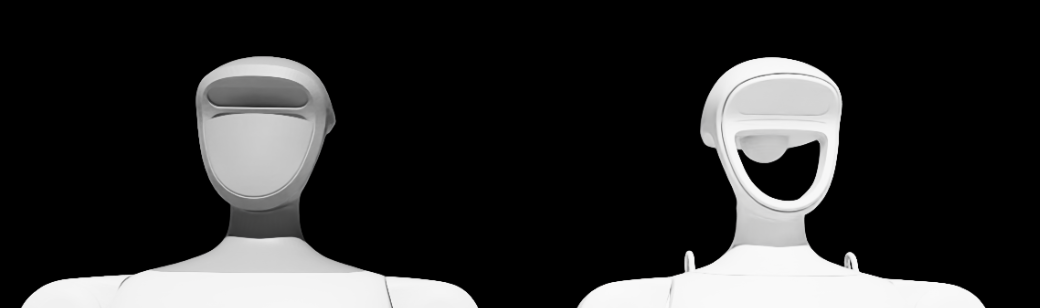
\includegraphics[width=0.75\linewidth]{immagini/g1_versions.png}
    \caption{G1 presente negli asset Isaac Sim e G1 disponibile online}
    \label{fig:confronto_g1}
\end{figure}

Il modello URDF del G1 è fornito in più varianti con diversi gradi di libertà, con o senza mani. La scelta è ricaduta sulla versione con dodici gradi di libertà corrispondenti alle articolazioni delle due gambe: due per ogni lato del bacino, una per ogni ginocchio e due per ciascuna caviglia. Selezionare un modello con le sole articolazioni dedicate alla locomozione ha permesso di evitare di introdurre variabili non utilizzate. Per completezza, nella tabella \ref{tab:g1_joint_link} si riporta la totalità di sistemi di riferimento e giunti presenti nel G1 ottenuto.

\begin{table}[h]
    \centering
    \begin{tabular}{|c|c|} 
        \hline
        \textbf{Sistemi di riferimento}& \textbf{Giunti}\\ \hline
        \textit{pelvis}(ospita i sensori)& ...\\ \hline
        \textit{left$\_$hip$\_$link}&\textit{left$\_$hip$\_$joint} \\ \hline
        \textit{left$\_$hip$\_$link}&\textit{left$\_$hip$\_$joint} \\ \hline
        \textit{left$\_$hip$\_$link}& \textit{left$\_$hip$\_$joint}\\ \hline
        \textit{left$\_$knee$\_$link}& \textit{left$\_$knee$\_$joint}\\ \hline
        \textit{left$\_$ankle$\_$link}& \textit{left$\_$ankle$\_$joint}\\ \hline
        \textit{left$\_$ankle$\_$link}& \textit{left$\_$ankle$\_$joint}\\ \hline
        \textit{right$\_$hip$\_$link}& \textit{right$\_$hip$\_$joint}\\ \hline
        \textit{right$\_$hip$\_$link}& \textit{right$\_$hip$\_$joint}\\ \hline
        \textit{right$\_$hip$\_$link}& \textit{right$\_$hip$\_$joint}\\ \hline
        \textit{right$\_$knee$\_$link}& \textit{right$\_$knee$\_$joint}\\ \hline
        \textit{right$\_$ankle$\_$link}& \textit{right$\_$ankle$\_$joint}\\ \hline
        \textit{right$\_$ankle$\_$link}& \textit{right$\_$ankle$\_$joint}\\ \hline
    \end{tabular}
    \caption{Sistemi di riferimento e rispettivi giunti}
    \label{tab:g1_joint_link}
\end{table}

\subsubsection{Implementazione dei sensori virtuali}
Accertata la correttezza dei giunti e dei relativi sistemi di riferimento, si è proceduto ad equipaggiare il robot con la sensoristica prevista. Come ampiamente descritto nel paragrafo 1.4.3, il G1 è provvisto di una camera RGB-D Realsense D435i e di un LiDAR Livox Mid-360. La ricerca di modelli URDF da convertire ha prodotto scarsi risultati per entrambi i sensori: del primo esistono poche versioni, mentre del secondo sono reperibili solo quelle compatibili con Gazebo\footnote{piattaforma di simulazione concorrente ad Isaac Sim}. Pur provando tutte le versioni disponibili del D435i, non è stato trovato un modello completamente compatibile e funzionante. Dunque, si è deciso di percorrere la strada più accettabile, almeno provvisoriamente, cioè l'adattamento allo scopo di dispositivi simili. Tra gli asset nella libreria di Isaac Sim è emerso il Realsense D455, l'evoluzione del D435i. Segue la tabella \ref{tab:realsense_comparison} che sottolinea le differenze tra le due camere RGB-D.

\begin{table}[h]
    \centering
    \begin{tabular}{|l|l|l|}
    \hline
    \textbf{Caratteristica}                 & \textbf{D435i} & \textbf{D455} \\   \hline
    Portata Ideale                           & 0.3 m - 3 m                   & 0.4 m - 6 m                  \\ \hline
    Accuratezza Profondità                   & $<$2\% a 2 m                    & $<$2\% a 4 m                   \\ \hline
    Min. Distanza Prof.                      & $\sim$0.1 m (10 cm) / 28 cm & $\sim$0.4 m (40 cm) / 52 cm \\ 
    \hline
    Tecnologia Sensore RGB                   & Rolling Shutter               & Global Shutter               \\ \hline
    Risoluzione RGB                          & 1920x1080                     & 1280x800                     \\  \hline
    FOV RGB (H x V)                          & 69° x 42°                     & 86° x 57° (o 90° x 65°)      \\   \hline
    Dimensioni                               & 90 mm x 25 mm x 25 mm         & 124 mm x 26 mm x 29 mm       \\ \hline
    \end{tabular}
    \caption{Confronto tra Intel RealSense D435i e D455}
    \label{tab:realsense_comparison}
\end{table}

Negli altri aspetti salienti come la presenza di IMU, la risoluzione della profondità o il valore degli FPS, i due prodotti sono identici e sfruttano le stesse tecnologie, motivo per cui si è deciso di modificare manualmente, via Isaac Sim, parte dei parametri discrepanti tra i due. Il modello virtuale è stato, dunque, montato sul robot nel sistema di riferimento \textit{d435$\_$link}, solidale alla testa e, a sua volta, nel sistema \textit{pelvis}. 

Per quanto riguarda il Mid-360, non sono presenti asset simili nella libreria, dunque si è preferito utilizzare il modello ideale di LiDAR offerto dal software e configurarlo completamente per rendere quanto più simile possibile al dispositivo originale. In particolare, i parametri interessati sono stati: FOV, risoluzione e distanza minima di rilevamento. Per contribuire alla robustezza del sistema, ogni parametro dipendente dalle condizioni ambientali è stato impostato seguendo lo scenario peggiore. Ad esempio, la distanza massima di rilevazione è stata quantificata in 40 m che, secondo la documentazione del prodotto, corrisponde al caso limite: un ambiente composto da superfici con il 10$\%$ di riflettività\footnote{proprietà che una superficie ha di riflettere radiazioni incidenti su di essa}.  In questo caso, il sistema di riferimento scelto per il montaggio è stato \textit{mid360$\_$link}, anch'esso in \textit{pelvis}.

Le caratteristiche dell'IMU non sono specificate nel datasheet del G1, dunque, si è implementato l'unico sensore disponibile nelle librerie, collocandolo nel rispettivo sistema di riferimento \textit{imu$\_$in$\_$torso} interno a \textit{pelvis}. Naturalmente, il robot è provvisto di encoder ai giunti, ma questi non vanno aggiunti nella simulazione perché sarà Isaac Lab stesso a controllare e monitorare gli attuatori. Aggiunti i tre sensori come descritto, il modello ottenuto è stato salvato in un file USD dedicato che verrà fornito al framework di simulazione in qualità di agente.


\subsection{Creazione degli scenari di simulazione}
\subsubsection{Scenario base}


\subsubsection{Scenario dinamico}


\subsubsection{Scenario complesso}


\subsection{Progettazione del Markov Decision Process}
\subsubsection{Azioni}
Nel Markov Decision Process, le azioni corrispondono alle variabili di output del modello e nel progetto sono dedicate al controllo dei dodici giunti delle gambe del robot. Le possibili grandezze manipolabili dall'agente sono: la posizione, la velocità e la forza. Il primo caso rappresenta un controllo ad alto livello che astrae parte della dinamica e si adatta a compiti che prevedono pose statiche e movimenti ben definiti. Il controllo in velocità è più diretto e utilizzato per la definizione di traiettorie nello spazio d'azione, ma richiede una conoscenza approfondita del singolo motore ed ha bisogno di un PID\footnote{controllo proporzionale, integrale e derivativo}. Il controllo in forza è quello più realistico ma il più difficile da attuare, richiede modelli avanzati che riescano a comprendere i legami dinamici ed i vincoli fisici intrinseci ai motori in modo da produrre uscite coerenti. Quest'ultima è l'opzione che è sembrata più aderente alla trattazione, seppur rendesse più complesso il compito.

\begin{table}[h]
    \centering
    \begin{tabular}{|c|c|}\hline
         \textbf{Azioni} & \textbf{Dimensioni}\\ \hline
         Forza ai giunti & (12,1)\\ \hline
    \end{tabular}
    \caption{Azioni dell'agente e rispettive dimensioni}
    \label{tab:act}
\end{table}

Utilizzare solo i giunti delle gambe ha permesso di ridurre la dimensione del tensore di uscita dalla rete e, dunque, di addestrare una politica che si concentrasse sullo spazio delle azioni che più impatta sulla locomozione. Controllare tutti i gradi di libertà del G1 avrebbe reso la trattazione più realistica poiché la locomozione, tanto quella umana quanto quella robotica, coinvolge anche le rotazioni del busto ed il movimento delle braccia per aumentare la fluidità e la stabilità. Questo, però, avrebbe reso l'addestramento più lungo e dispendioso, senza garanzia di una maggiore efficacia.

% completare magari con riferimenti scientifici

%tabella delle azioni


\subsubsection{Osservazioni}
Le osservazioni compongono una larga parte degli ingressi della rete e servono a creare un modello dell'ambiente con cui l'agente interagisce. Non corrispondono alle sole misurazioni dei sensori, ma anche alla modellazione del compito assegnato che, nel caso specifico, è la posizione dell'obiettivo nello spazio.

% completare 

%aggiornare
\begin{table}[h]
    \centering
    \begin{tabular}{|c|c|}
    \hline
    \textbf{Osservazioni} & \textbf{Dimensioni} \\ \hline
    Posizione dei giunti & (12, 1) \\ \hline
    Velocità dei giunti & (12, 1) \\ \hline
    Velocità IMU & (3, 1) \\ \hline
    Accelerazione IMU & (3, 1) \\ \hline
    Immagine RGB & (192, 108, 3) \\ \hline
    Immagine Depth & (192, 108, 1) \\ \hline
    Lidar & (6144, 1) \\ \hline
    Target & (4, 1) \\ \hline
    \end{tabular}
    \caption{Osservazioni e rispettive dimensioni}
    \label{tab:obs}
\end{table}

% feature extraction 

\subsubsection{Ricompense}
Le ricompense, nel Markov Decision Process, rappresentano il feedback dell'ambiente rispetto alle azioni dell'agente. La loro modellazione risulta un compito complesso perché richiede la valutazione accurata dell'impatto di ciascuna sull'apprendimento della politica ottimale. Le ricompense risultano, di fatto, degli iperparametri il cui tuning richiede tempo e addestramenti. 

% riferimento a stato dell'arte

% aggiornare
\begin{table}[h]
    \centering
    \begin{tabular}{|c|c|}
    \hline
    \textbf{Ricompense} & \textbf{Peso} \\ \hline
    Vivo & [DA IMPL] \\ \hline
    In piedi & [DA IMPL] \\ \hline
    Caduto & [DA IMPL] \\ \hline
    Cammina & [DA IMPL] \\ \hline
    Uscita dallo spazio operativo & [DA IMPL] \\ \hline
    Collisione con un ostacolo & [DA IMPL] \\ \hline
    Avvicinamento all'obiettivo (soft) & $1-\tanh$ \\ \hline
    Avvicinamento all'obiettivo (hard) & proporzionale \\ \hline
    Obiettivo raggiunto & [DA IMPL] \\ \hline
    \end{tabular}
    \caption{Ricompense e rispettivi pesi}
    \label{tab:rew}
\end{table}


\subsubsection{Eventi}
% eventi

% aggiornare
\begin{table}[h]
    \centering
    \begin{tabular}{|c|c|}
    \hline
    \textbf{Eventi} & \textbf{Modalità} \\ \hline
    Uscita dallo spazio operativo & reset \\ \hline
    Collisione con un ostacolo & reset \\ \hline
    Caduta del robot & reset \\ \hline
    Obiettivo raggiunto & reset \\ \hline
    \end{tabular}
    \caption{Eventi e rispettive modalità di gestione}
    \label{tab:ev}
\end{table}


\subsubsection{Terminazioni}
% terminazioni

% aggiornamento
\begin{table}[h]
    \centering
    \begin{tabular}{|c|c|}
    \hline
    \textbf{Terminazioni}\\\hline
    Fine del tempo\\ \hline
    Caduta del robot\\ \hline
    Uscita dallo spazio operativo\\ \hline
    Collisione con un ostacolo\\ \hline
    Obiettivo raggiunto\\ \hline
    \end{tabular}
    \caption{Terminazione degli episodi}
    \label{tab:term}
\end{table}


\subsection{Scrittura del codice}


\subsection{Esecuzione dell'addestramento}
\subsubsection{Pianificazione}
Per permettere uno sviluppo modulare e un corretto debug, si è pianificata una roadmap di addestramenti per di complessità incrementale. La difficoltà crescente


\subsubsection{Tuning degli iperparametri}


\subsubsection{Impostazioni}
La parametrizzazione rimanente non è rivolta al miglioramento delle prestazioni del modello, ma alla leggibilità dei risultati e all'ottimizzazione delle risorse per l'addestramento. 

% video 

% numero di ambienti 

% etc